\documentclass[11pt,show 
notes,notheorems,noamsthm,blank]{beamer} % default is 11pt
\usetheme{metropolis}
% \usepackage{beamerthemeshadow}
% \usepackage{times}
\usepackage[utf8]{inputenc}
\usepackage[scaled]{helvet} % ss
\usepackage[T1]{fontenc}
\usepackage{eurosym}
\usepackage{graphics, graphicx}
\usepackage{url}
% \usepackage{multirow}
\usepackage{listings}
\usepackage{epsfig}
%  \usepackage[portuguese]{babel}
%  \usepackage[latin1]{inputenc}  
\usepackage{fancyvrb}
\usepackage[prefix=tikzsym]{tikzsymbols}

\usepackage{fontawesome}
% \usepackage{xcolor}


% \usepackage[marvosym]{tikzsymbols}
% \usepackage{rotating}
% \usepackage{subfigure}
% \usepackage{default}
 \usepackage{algorithmic}
 \usepackage{algorithm}
\usepackage{rotating}
\usepackage{hyperref}
\definecolor{links}{HTML}{FF5050}
\definecolor{inlinks}{HTML}{4D94FF}
\hypersetup{colorlinks,linkcolor=inlinks,urlcolor=links}
\beamertemplatetransparentcovered
%  \usepackage[portuguese]{babel}
%  \usepackage[latin1]{inputenc}  
\usepackage{rotating}
\usepackage{colortbl}
% \usepackage{moreverb}
% \usepackage{tikz}
% \usepackage{wrapfig}
\setbeamertemplate{bibliography item}{\insertbiblabel}
% \usepackage{tikz}
% \usetikzlibrary{arrows,positioning,shapes}
% \usetikzlibrary{shapes,calc,shadows}
\pgfdeclarelayer{background}
\pgfdeclarelayer{foreground}
% \pagestyle{fancy}
\pgfsetlayers{background,main,foreground}
\usepackage{url}
\usepackage{hyperref}
% \usepackage{color}X
\setbeamertemplate{navigation symbols}{}
% \renewcommand{\algorithmicrequire}{\textbf{Input:}}
% % \renewcommand{\algorithmicensure}{\textbf{Output:}}
% \hypersetup{
%     colorlinks,%
%     citecolor=BrickRed,%
%     filecolor=black,%
%     linkcolor=blue,%
%     urlcolor=BrickRed
% }





\usepackage{tikz}
\usetikzlibrary{calc,shapes.symbols,shapes.geometric,positioning,arrows,chains}
\usetikzlibrary{backgrounds,decorations,decorations.text,
decorations.pathreplacing}
% tiks definitions
\usetikzlibrary{arrows.meta}
\tikzstyle{default_rectangle} = [black, fill=white]
\tikzset{>=stealth}
\tikzset{every picture/.append style={font=\small}}
\usetikzlibrary{arrows, matrix, shadows}
\tikzset{>=stealth}
\tikzstyle{every picture}=[line width=0.75pt]
\tikzstyle{every instance}=[font=\small]
\tikzstyle{default_rectangle} = [black, fill=white]
\definecolor{myblue}{RGB}{68,119,170}
\definecolor{myred}{RGB}{204,102,119}
\definecolor{mygreen}{RGB}{17,119,51}
\definecolor{myyellow}{RGB}{221,204,119}
% Definitions for figures
\tikzstyle{server}=[circle,draw,minimum size=2em,scale=.9,solid,fill=green!20]
\tikzstyle{site}=[circle,draw,minimum size=2em,scale=.9,solid,fill=red!20]
\tikzstyle{root}=[circle,draw,minimum size=2em,scale=.9,solid,fill=red!20]
\tikzstyle{user}=[circle,draw,minimum size=2em,scale=.9,solid,fill=yellow!20]
\tikzstyle{cache}=[rectangle,draw,minimum 
size=3em,scale=.9,solid,fill=blue!20,minimum height=1em]

% Definitions for figures
\tikzstyle{server}=[circle,draw,minimum size=2em,scale=.9,solid,fill=green!20]
\tikzstyle{site}=[circle,draw,minimum size=2em,scale=.9,solid,fill=red!20]
\tikzstyle{root}=[circle,draw,minimum size=2em,scale=.9,solid,fill=red!20]
\tikzstyle{user}=[circle,draw,minimum size=2em,scale=.9,solid,fill=yellow!20]
\tikzstyle{cache}=[rectangle,draw,minimum 
size=3em,scale=.9,solid,fill=blue!20,minimum height=1em]


\usepackage{pgf}
\pgfdeclareimage[height=0.5cm]{logo}{fig/sidn-delft}
% \addtobeamertemplate{navigation symbols}{}{%
%     \usebeamerfont{footline}%
%     \usebeamercolor[fg]{footline}%
%     \hspace{1em}%
%     \insertframenumber/\inserttotalframenumber
% }

% \setbeamercolor{footline}{fg=blue}
\setbeamerfont{footline}{series=\bfseries}


% \setbeamerfont{}{family=\rmfamily,series=\bfseries,size={\fontsize{12}{36}}}

%  \logo{\pgfuseimage{logo}}

\begin{document}
\title{draft-moura-dnsop-authoritative-recommendations-04}  
\author[Moura et. al]{\textbf{Giovane C. M. Moura}$^{1,2}$, Wes Hardaker$^3$, 
\\John Heidemann$^3$, Marco Davids$^1$\\}
\vspace{-0.3cm}
\institute{$^1$SIDN Labs, $^2$TU Delft, $^3$USC/ISI\\
%    \includegraphics[width=9cm]{fig/logos.png}
}


   
   
\date {DNSOP -- IETF 105\\Montreal, CA\\
2019-07-23\\


}  

\frame{\titlepage} 






\begin{frame}
\frametitle{Draft History}


\begin{itemize}


% \item This is an \textbf{Informational} draft 
\item  First time presented at DNSOP  @ IETF103
    \begin{itemize}
     \item Video: \begin{tiny} \url{https://www.youtube.com/watch?v=l2ixYuwuaqY} \end{tiny}
     \item Slides: \tiny  \url{https://datatracker.ietf.org/meeting/104/materials/slides-104-dnsop-dnsop-authoritative-recommendations-01.pdf}
    \end{itemize}
    
\item Today: -04 
\begin{itemize}
 \item   \begin{tiny}  \url{https://datatracker.ietf.org/doc/draft-moura-dnsop-authoritative-recommendations/04/} \end{tiny}
\end{itemize}

\item All changes are documented in the text and on Github:
\begin{itemize}
 \item \begin{tiny}  \url{https://github.com/gmmoura/draft-moura-dnsop-authoritative-recommendations/issues} \end{tiny}
\end{itemize}



% \item Before we show the changes: \textbf{thanks folks }for all your comments @103 in Prague

% \begin{itemize}
%   \item Even if I did not seem to agree there, most of folks were right once I watched the video and though it through
%   \end{itemize}

% \item Today: covering most important  issues (others on Github, fixed)

\end{itemize}
\end{frame}




\begin{frame}
\frametitle{Draft History}


\begin{itemize}

% 
% % \item This is an \textbf{Informational} draft 
% \item  First time presented at DNSOP  @ IETF103
%     \begin{itemize}
%      \item Video: \begin{tiny} \url{https://www.youtube.com/watch?v=l2ixYuwuaqY} \end{tiny}
%      \item Slides: \tiny  \url{https://datatracker.ietf.org/meeting/104/materials/slides-104-dnsop-dnsop-authoritative-recommendations-01.pdf}
%     \end{itemize}
%     
% \item Today: -04 
% \begin{itemize}
%  \item   \begin{tiny}  \url{https://datatracker.ietf.org/doc/draft-moura-dnsop-authoritative-recommendations/04/} \end{tiny}
% \end{itemize}
% 
% \item All changes are documented in the text and on Github:
% \begin{itemize}
%  \item \begin{tiny}  \url{https://github.com/gmmoura/draft-moura-dnsop-authoritative-recommendations/issues} \end{tiny}
% \end{itemize}
% 


\item Before we show the changes: \textbf{thanks folks }for all your comments @103 in Prague

\begin{itemize}
  \item Even if I did not seem to agree there, most of folks were right once I watched the video and though it through
  \end{itemize}

\item Today: covering most important  issues (others on Github, fixed)

\end{itemize}
\end{frame}

\begin{frame}
\frametitle{Changes from -03}
\begin{block}{ Issue \#14: \texttt{s/Recommendations/Considerations/}}
\begin{itemize}
 \item Liman pointed at 103 that the word ``recommendations'' is too strong
 \begin{itemize}

 \item Could reduce  setups heterogeneity 
 \end{itemize}
 \item So we replace it by ``considerations''
 \item "Considerations" also used on other DNS RFCs (5395,6135,6895,7626)

  \item Note to self: 
  \begin{itemize}
   \item \texttt{IETF(Recommendation) != Paper(Recommendation)} 
   \item \texttt{Papers(Recommendation) $\simeq$ IETF(Consideration)}
 
  \end{itemize}

\end{itemize}

 
\end{block}



\end{frame}


\begin{frame}
\frametitle{Changes from -03}
\begin{block}{ Issue \#13: Draft mostly about anycast, but not exclusively}
\begin{itemize}
 \item Joe Abley pointed that except for the TTL consideration, all the others are related to anycast
 \item He is right
 \item Our fix:
 \begin{itemize}
 
 \item
 
%   \item \begin{verbatim}
      \texttt{``It is likely that these considerations might be useful in a wider context,
         such as for any stateless/short-duration, anycasted service. 
         Because the conclusions of the studies don't verify this fact, 
         the wording in this document discusses DNS authoritative services only.''}
%         \end{verbatim}

 \end{itemize}
%  \item Why? \texttt{``claims without evidence can be dismissed without evidence''}
\end{itemize} 

 
\end{block}



\end{frame}



\begin{frame}
\frametitle{Changes from -03}
\begin{block}{ Issue \#17: TTL considerations controversy }
\begin{itemize}
\item Peter Koch pointed how complex the issue was (and it was tried 15 years ago)
\item He says TTLs is for zone maintainers, not DNSOPs 
\begin{itemize}
 \item Not true for all cases: many TLDs ops run their own DNSs as well, their parent TTLs may affect their child delegations TTLs
 
\end{itemize}
\item Our fix:
\begin{enumerate}
 \item Rewritten  it completely (highlighting issues pointed by Peter)
 \item New study (Moura19a) on TTLs (presented at IEPG) that covers most issues
%  \item 
\end{enumerate}

\end{itemize} 

 
\end{block}
\end{frame}




\begin{frame}
\frametitle{Changes from -03}
\begin{block}{ Issue \#15: Paper selection could be more diverse}
\begin{itemize}
%  \item Joe Abley pointed that except for the TTL consideration, all the others are related to anycast
%  \item He is right
%  \item Our fix:
\item 3 papers (not by the authors) added to references
\item Also, paper's related work sections cover it
\item \texttt{``This document describes the key engineering options, and points readers to the pertinent papers for details and other research works related to each recommendation here presented.''}
%  \begin{itemize}
%  
%  \item
%  
% 
% 
%  \end{itemize}
%  \item Why? \texttt{``claims without evidence can be dismissed without evidence''}
\end{itemize} 

 
\end{block}
\end{frame}



\begin{frame}
\frametitle{Changes from -03}
\begin{block}{ Issue \#12: Ripe Atlas bias on Consideration on anycast locations (C3)}
\begin{itemize}
%  \item Joe Abley pointed that except for the TTL consideration, all the others are related to anycast
%  \item He is right
%  \item Our fix:
\item George Michaelson pointed that the ``view of Atlas is biased to Europe" in C3
\item The paper, however, show results \textit{per region and country} (not mentioned in -03)
% \item Our fix:



\end{itemize} 

\end{block}
\vspace{-0.5cm}

\begin{figure}
\centering
   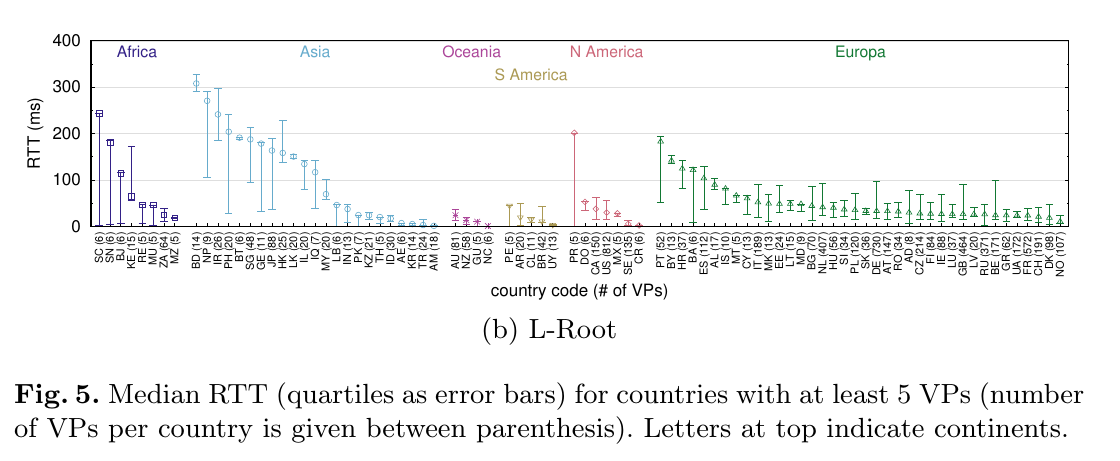
\includegraphics[width= 9cm]{rtt-schmidt17a.png}
\end{figure}

\end{frame}

\begin{frame}
\frametitle{Changes from -03}
\begin{block}{ Issue \#12: Ripe Atlas bias on Consideration on anycast locations (C3)}



\begin{itemize}
\item Our fix: \texttt{``Given that Atlas has better coverage in Europe than other regions, the authors specifically analyzed results per region and per country (Figure 5 in [Schmidt17a]), and show that Atlas bias to Europe does not change the conclusion that location of anycast instances dominates latency.''}

\item Also, the study has been peer-reviewed
\end{itemize}

\end{block}
\end{frame}


\begin{frame}
 \frametitle{Questions?}
 
 \begin{itemize}
  \item Questions?
  \item Draft future?
 \end{itemize}

 
 
\end{frame}


% 
%  \begin{frame}[allowframebreaks] {References}
%  \small
% \bibliographystyle{IEEEtran}
% % \balance
% \small
% \bibliography{subset,rfc}
% \end{frame}
%  
\end{document}
